
\section{Obiettivo}

Il mio compito nello sviluppo dell'applicazione è stato quello 
di creare un \textbf{prototipo} iniziale avendo a disposizione un mock up creato con
proto.io\cite{protoio} e una serie di requisiti essenziali.

\section{Requisiti essenziali}

La base di partenza di QIX sono state delle funzionalità essenziali e 
sonstanzialmente molto difficili da inserire in una versione dell'app già avanzata.
È stati quindi deciso di creare un prototipo di partenza avente i seguenti requisiti:

\begin{itemize}
    \item {
        \textbf{Navigazione dinamica}: L'applicazione deve gestire dei cambiamenti di contesto
        dinamici: dev'essere possibile mostrare all'utente contenuti dinamici indipendentemente
        dal contesto in cui si trova. 
    }
    \item {
        \textbf{QIX Shake}: L'utente deve poter agitare lo smartphone in qualsiasi
        sezione dell'applicazione e il risultato deve essere basato sul contesto attuale o su delle direttive dettate
        da delle Rest API;
    } 
    \item {
        \textbf{Animazioni interattive}: L'intera applicazione dev'essere progettata in modo tale da presentare all'utente
        delle \textbf{animazioni interattive} in stile CardView\cite{cardview} disponibili in 
        qualunque sezione o vista in cui si trovi l'utente e definite dal contesto attuale;

        Le animazioni in questione devono essere progettate in pagine, in cui ogni pagina può contenere 
        più CardView. L'utente vedrà in un determinato momento una e soltanto una pagina.

        Ogni CardView deve essere trascinabile dall'utente e deve interagire con le altre CardView della pagine. 
        Quando l'utente usa una forza di trascinamento superiore a un valore di soglia tutte le viste devono
        cadere per gravità;
        
        Tale gravità finirà con la fine dell'animazione o l'apparizione di una nuova pagina se presente;
    }
    \item {
        \textbf{Autenticazione}: L'applicazione deve supportare tre diversi stati o modalità di autenticazione:
        \begin{enumerate}
            \item\textbf{Trial Mode}: l'utente è anonimo, esiste solo un id per tenere traccia dei suoi QIX coins.
            \item\textbf{Signed Mode}: l'utente ha inserito il numero di telefono e il suo genere;
            \item \textbf{Pro Mode}: l'utente aggiunge dei dati su se stesso o collega il suo account a dei social media come Facebook, Google o Instagram;
        \end{enumerate}
        Si nota facilmente che non esiste una stato in cui l'utente non è registrato: questo perchè
        per tenere traccia dei suoi QIX coins e di altri dati utili è necessario avere una riferimento all'utente;
    }
    \item {
        \textbf{DeepLinks}: L'applicazione deve poter essere avviata dinamicamente
        attraverso dei \textbf{Deep Links}\cite{deeplinks};
        E deve essere in grado di gestirli in base al contesto dell'utente;
    }
\end{itemize}

% \section{La navigazione dinamica}

% % Analizzando il requisito mi sono posto diverse domande: \\ \\
% % \noindent{
% %     \large\textit{Cosa significa dinamicamente?}
% %     \normalsize{Il nostro obiettivo in questo caso è mostrare all'utente \textbf{contenuti diversi}
% %     indipendentemente dal constesto e quindi dalla vista in cui si trova}\\ \\
% %     \large\textit{Quale contesto?}
% %     \normalsize{Con contesto dell'utente si intende lo stato attuale dell'applicazione,
% %     quindi l'intero stack di navigazione se presente;
% %     } \\ \\
% % }

% Prima di entrare nel merito della soluzione al problema, elenco brevemente gli
% standard di navigazione delle app iOS.

% Ogni applicazione può avere degli \textbf{UINavigationController}\cite{navigationcontroller},
% ossia dei contenitori di \textbf{UIViewController}\cite{viewcontroller} che vengono
% utilizzati per mantenere lo stack di navigazione e gestire la transizioni tra due UIViewController.

% Nella figura~\ref{fig:1} si nota facilmente come il Navigation controller gestisce un'array di View Controller e una sola 
% navigation bar. 
% In iOS sono infatti innate molte animazioni di navigazione che è utile sfruttare, piuttosto di creare 
% componenti custom poi difficili da rendere interattivi.\\

% \begin{minipage}{\linewidth}
%     \centering
%     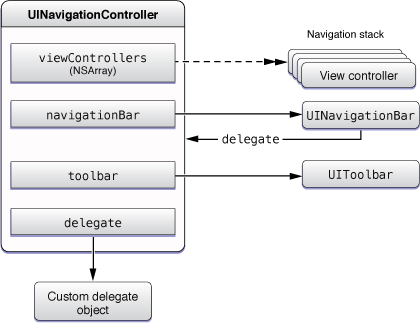
\includegraphics[width=5cm]{navigation}
%     \captionof{figure}{Navigation controller scheme}
%     \label{fig:1}
% \end{minipage}

% \subsection{Tipologie di navigazione}\label{sec:navigation}

% Esistono tre tipologie base di navigazione:

% \begin{enumerate}
%     \item{\textbf{Push}: un UIViewController avente un navigation controller può rendere
%     visibile un altro ViewController attraverso la funzione "pushViewController" di un Navigation controller\par
%     \begin{minipage}{\linewidth}
%         \centering
%         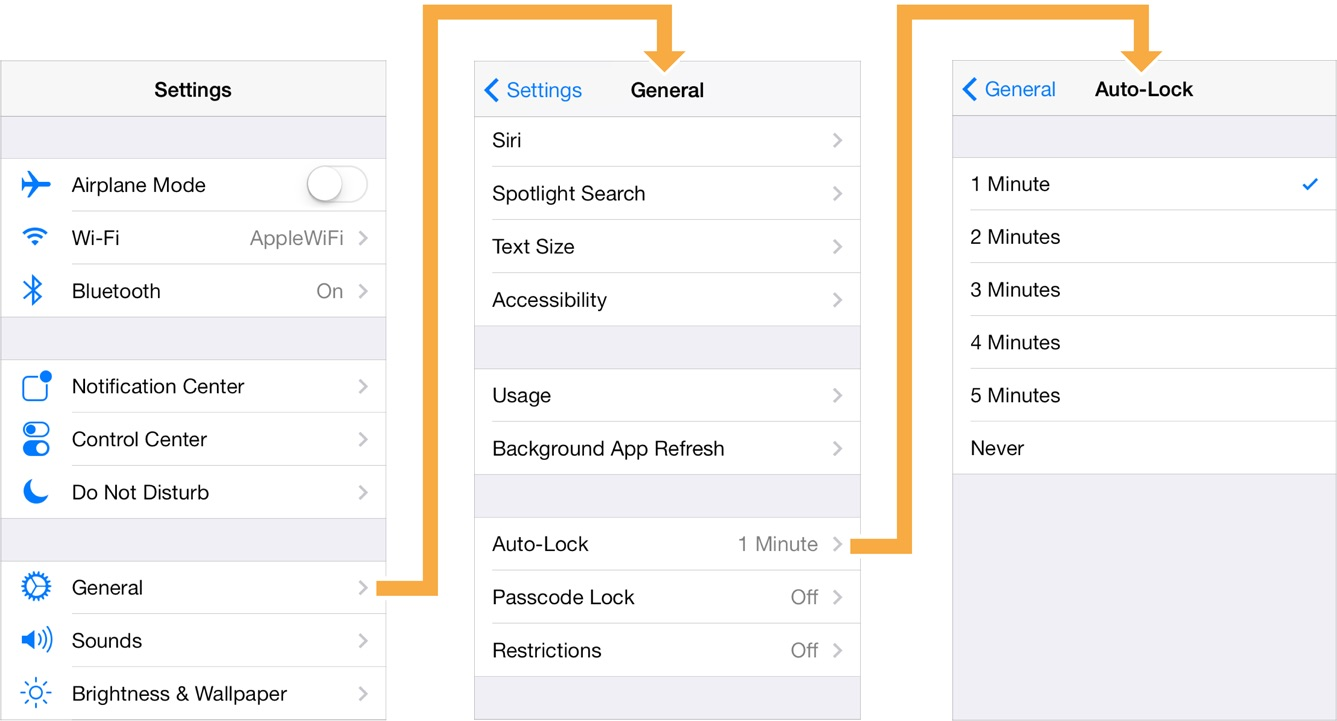
\includegraphics[width=10cm]{push}
%         \captionof{figure}{Presantazione di un ViewController tramite push}
%         \label{fig:2}
%     \end{minipage}
%     }
%     \item{ \textbf{Modal}: un ViewController può presentare un altro ViewController senza necessariamente avere un 
%         Navigation Controller, l'animazione standard è dal basso verso l'alto come in figura~\ref{fig:3}\par
%         \begin{minipage}{\linewidth}
%             \centering
%             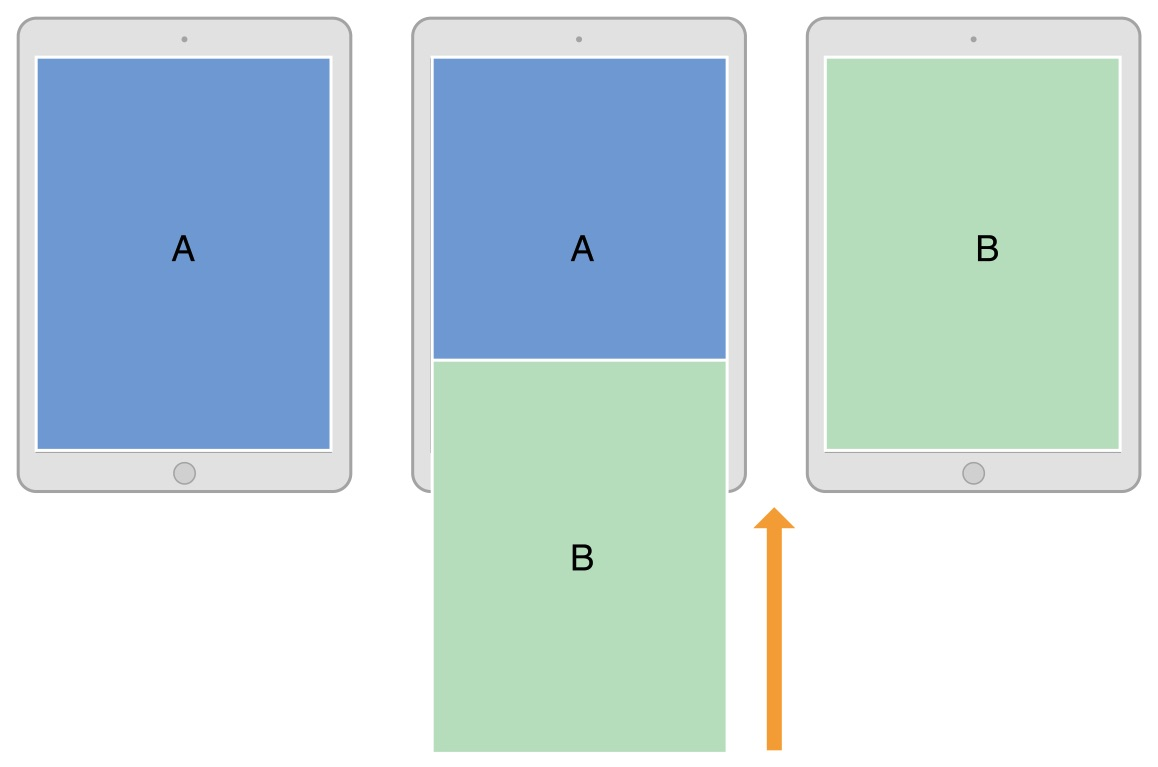
\includegraphics[width=10cm]{modal}
%             \captionof{figure}{
%                 Presantazione di un ViewController tramite modal
%             }
%             \label{fig:3}
%         \end{minipage}
%     }
%     \item{\textbf{Segue}: Una segue non è altro che un link tra due view controller attraverso un'interfaccia
%         grafica. In base alla tipologia cambia il tipo di navigazione (Modal o Push)
%     }
% \end{enumerate}

% Avendo definito i principali metodi di navigatione tra ViewController torniamo al problema iniziale:
% \textit{Come possiamo rendere dinamica la navigazione?}

% A seguito di uno studio approfondito di varie tecniche di navigazione iOS ho scelto di utilizzare il
% \textbf{Coordinator Pattern}\cite{coordinatorpattern}.

% \subsection{Il Coordinator Pattern}

% Generalmente in iOS l'intera logica di un ViewController viene scritta nel ViewController stesso, creando spesso
% file di grosse dimensioni e disordine generale. Il Coordinator Pattern è nato proprio per rendere 
% le applicazioni più scalabili e leggere. 

% Ogni ViewController infatti delega tutte le decisioni al suo Coordinator che in base a determinate logiche deciderà
% i passi successivi.

% Ogni Coordinator può controllare un ViewController o più Coordinator, questo rende le viste
% indipendenti tra di loro e rende ogni ViewControler totalmente invisibile agli altri.\\

% \begin{minipage}{\linewidth}
%     \centering
%     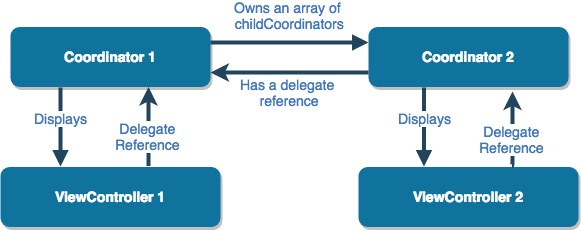
\includegraphics[width=10cm]{coordinator}
%     \captionof{figure}{
%         Il Coordinator Pattern
%     }
%     \label{fig:4}
% \end{minipage}\\ \\

% La resposibilità dei coordinator è infatti la navigazione, come un navigation controller gestisce i sui View Controller, un coordinator gestisce
% i suoi figli e questo rende ogni vista o flow di navigazione totalmente indipendente dal resto dell'applicazione.

% Per navigare tra i view controller vengono generalmente usate le tipologie di navigazione
% descritte nella sezione~\ref{sec:navigation}, tranne le segue, che essendo definete da vista grafica renderebbero
% la navigazine statica e fissata su determinati ViewController. \\

% Di seguito in figura~\ref{fig:5} presento uno schema dell'utilizzo di due coordinator
% per la gestione di una lista di prodotti e il carrello. \\

% \begin{minipage}{\linewidth}
%     \centering
%     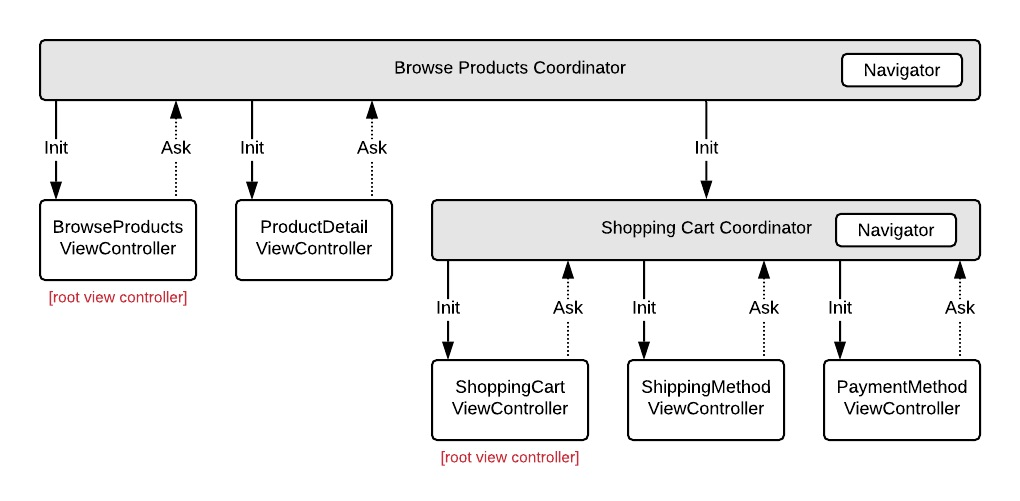
\includegraphics[width=10cm]{coordinator-example}
%     \captionof{figure}{
%        Esempio di coordinator pattern
%     }
%     \label{fig:5}
% \end{minipage}\\ \\

% Come si evince dall'immagine è presente in entrambi i coordinator è presente un oggetto
% \textbf{navigator} che sarà in gestore di un UINavigationController

% \section{Il QIX Shake}

% In iOS ogni UIViewController risponde a degli eventi. L'evento designato per lo shake è
% \begin{minted}{swift}
%     func motionEnded(_ motion: UIEvent.EventSubtype,
%         with event: UIEvent?)
% \end{minted}

% In caso di shake infatto motion sarà uguale a .motionShake
% Per rendere disponibile l'evento "shake" in un qualunque ViewController la soluzione è stata abbastanza semplice:
% è bastato l'utlizzo di un ViewController Genitore e attrvaerso l'eriditarietà ogni view controller è in grado
% di eseguire la stessa funzionalità.

% In questo caso è stato optato l'utilizzo delle notifiche locali: quando avviene uno shake i view controller inviano una notifica 
% globale e solo gli observer vi hanno accesso.

% \section{Le animazioni interattive}

% Per semplicità divido il requisito in diversi punti e per ognuno ne spiego la soluzione
% o metodologia utilizzata:

% \begin{enumerate}
%     \item\label{animationenum:1} Le animazioni devono essere disponibili in qualunque sezione o vista in cui si trovi l'utente e definite dal contesto attuale;

%     \item\label{animationenum:2} Ogni CardView deve essere trascinabile dall'utente;
    
%     \item\label{animationenum:3} Quando l'utente usa una forza di trascinamento superiore a un valore di soglia tutte le viste devono
%         cadere per gravità;

%     \item\label{animationenum:4} Ogni CardView mostrerà un contenuto dinamico differente e definito da dei componenti
%     limitati specifici

%     \item\label{animationenum:5} Le animazioni in questione devono essere progettate in pagine, in cui ogni pagina può contenere 
%     più CardView. L'utente vedrà in un determinato momento una e soltanto una pagina. 
%     Una volta che le CardView acquisisco una gravità e cadono, finirà l'animazione o apparirà
%     una nuova pagina, se presente;

%     \item\label{animationenum:7} Ogni CardView deve interagire con le altre della stessa pagina, come se si toccassero;

% \end{enumerate}

% % % % % % % % % % % % % % % % % % % % % % % % % % % % % % % % % % % % % %
% %                      Onnipresenza delle animazioni                    %
% % % % % % % % % % % % % % % % % % % % % % % % % % % % % % % % % % % % % %
% \subsection{~\ref{animationenum:1}. Onnipresenza delle animazioni}

% \textbf{Premessa}: il contenuto di ogni applicazione iOS è inserito all'interno di un oggetto denominato
%     \textbf{UIWindow}\cite{uiwindow}. Questa finestra è disponibile in ogni UIViewController e permette di aggiungere contenuti
%     come viste o interi UIViewController al di sopra di tutto il contesto dell'app. Questo rende essenzialmente ogni contenuto presentato
%     indipendente per esempio da un stack di navigazione.\\ 

% Per creare animazioni definite dal contesto usiamo quindi un semplice UIViewController che gestirà tutte le animazioni,
% ma invece di presentarlo attraverso i metodi base visti alla sezione~\ref{sec:navigation}, lo presentiamo al di sopra della UIWindow,
% in modo da non essere vincolati dal contesto dell'utente quando l'animazione finirà, ma allo stesso tempo
% consente di controllare l'inizializzazione di questo UIViewController in base al contesto.

% % % % % % % % % % % % % % % % % % % % % % % % % % % % % % % % % % % % % %
% %                        CardView trascinabile                          %
% % % % % % % % % % % % % % % % % % % % % % % % % % % % % % % % % % % % % %
% \subsection{~\ref{animationenum:2}. Aggiunta di una gesture}

% In iOS per interagire con le viste attraverso il display touch screen si utilizzano delle UIGestureRecognizer.
% Tali strumenti sono nativi e offrono diverse tipologie per l'iterazione:
% \begin{itemize}
%     \item UITapGestureRecognizer: respansabile della gestione dei tap

%     \item UIPinchGestureRecognizer: respansabile della gestione del pitch ossia la gesture spesso usata per lo zoom
    
%     \item UIRotationGestureRecognizer: respansabile della gestione delle rotazioni
    
%     \item UISwipeGestureRecognizer: responsabile di uno swipe ossia un trascinamento in una direzione molto breve
    
%     \item UIPanGestureRecognizer: responsabile del drag and drop
    
%     \item UIScreenEdgePanGestureRecognizer: responsabile di uno swipe ossia un trascinamento nei bordi dello schermo
    
%     \item UILongPressGestureRecognizer: responsabile di una prossione prolungata nel tempo
% \end{itemize}

% Per un'animazione che ha necessità di muoversi come se l'utente la stesse spostando occore una UIPanGestureRecognizer.
% Dalla doumentazione delle UIGestureRecognizer viene spiegato che ohni vista "draggabile" necessiata una gesture,
% per questo ogni card view dovrà averne una.

% % % % % % % % % % % % % % % % % % % % % % % % % % % % % % % % % % % % % %
% %                        Gravità                                        %
% % % % % % % % % % % % % % % % % % % % % % % % % % % % % % % % % % % % % %
% \subsection{UIKit Dynamics: Cos'è e gli strumenti di base}

% Per la progettazione iniziale delle animazioni è stato fatto un attento studio a metodologie e frameworks
% atti a creare animazioni interattive fluide.

% Alla fine è stato deciso di utilizzare un pacchetto
% nativo di iOS incluso nello UIKit\cite{uikit}, chiamato UIKit Dynamics\cite{uidynamics}: questo framework,
% con una serie di API, offre delle funzioni di animazione base che 
% includo la fisica del mondo reale.

% Il framework si basa su degli oggetti \textbf{UIDynamicAnimator}, ogni animator è responsabile delle
% animazioni che avengono sulla \textbf{referenceView} e si inizializza 
% attraverso la seguente funzione:

% \begin{minted}{swift}
%     UIDynamicAnimator.init(referenceView view: UIView)
% \end{minted}

% una volta inizializzato attraverso la funzione addBehavior sarà posibile assegnargli
% dei comportamenti fisici predefiniti. I comportamenti di base sono:

% \begin{itemize}
%     \item\textbf{UIDynamicBehavior}: il comportamento base da cui ereditano tutti gli altri;
%     \item\textbf{UIAttachmentBehavior}: crea una relazione o legame tra due DynamicItem o tra un DynamicItem e un punto di ancoraggio;
%     \item\textbf{UICollisionBehavior}: un oggetto che conferisce a un array di DynamicItems la possibilità di impegnarsi in collisioni tra loro e con i limiti specificati del comportamento
%     \item\textbf{UIFieldBehavior}: un oggetto che conferisce delle proprietà magnetiche, elettriche a un DynamicItem;
%     \item\textbf{UIGravityBehavior}: aggiunge all'oggeto un forza di gravità;
%     \item\textbf{UIPushBehavior}: Aggiunge all'oggetto una forza continua o istantanea in una direzione specifica;
%     \item\textbf{UISnapBehavior}: Un comportamento simile a una molla il cui movimento iniziale viene smorzato nel tempo in modo che l'oggetto si stabilizzi in un punto specifico.
% \end{itemize}

% Di seguito un esempio di implementazione degli strumenti UIDynamics in QIX

% \begin{minipage}{\linewidth}
%     \centering
%     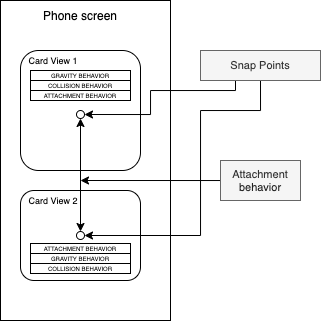
\includegraphics[width=10cm]{animation}
%     \captionof{figure}{
%        Schema dell'implementazione di UIDynamics
%     }
%     \label{fig:6}
% \end{minipage}\\

% % % % % % % % % % % % % % % % % % % % % % % % % % % % % % % % % % % % % %
% %                        Gravity                                     %
% % % % % % % % % % % % % % % % % % % % % % % % % % % % % % % % % % % % % %
% \subsection{~\ref{animationenum:3}. Aggiunta della gravità }

% Attraveso la UIPanGesture è possibile calcolare il vettore della velocità del trascinamento,
% con questo semplice dato e ciò che abbiamo studiato dello UIKit Dynamics è possibile aggiungere una gravità solo se
% il vettore della velocità è superiore a una soglia prestabilita.

% Per implementarlo è stato utilizzato un UIGravityBehavior, inizializzato in questo modo:

% \begin{minted}{swift}
%     let gravityBehavior = UIGravityBehavior(items: page.views)
%     gravityBehavior.magnitude = Constants.gravity
% \end{minted}

% Il valore \textbf{magnitude} è la forza di gravità che vogliamo
% assegnare alle viste in questione. \\

% Nella figura~\ref{fig:6} si vede lo schermo di uno smartphone, che presenta l'animazione
% voluta in questo caso con due CardView. Ognuna di esse ha un \textbf{UIAttachmentBehavior} al
% centro per fare in modo che sia sempre centrata in esso (o nel punto di drag dell'utente),
% un \textbf{UICollisionBehavior} per permettere che durante il drag le CardView possa scontrarsi e non si accavallino e un \textbf{UIGravityBehavior}, il quale 
% viene utilizzato per la caduta delle viste alla fine dell'animazione o al cambiamento di pagina.

% In più esiste uno speciale UIAttachmentBehavior tra i centri delle due CardView per permettere che il movimento di una
% sposti anche l'altra, è una sorta di corda che le lega.

% Per l'ingresso invece è stato inserito un UISnapBehavior, al centro per ogni oggetto, che anima 
% gli oggenti dando un effetto a molla.

% Tutte le animazione sono attivate e disattive in specifici momenti, questo dipende 
% dalla UIPanGestureRecognizer e dai movimenti dell'utente.

% % % % % % % % % % % % % % % % % % % % % % % % % % % % % % % % % % % % % %
% %                        Modular CardView                               %
% % % % % % % % % % % % % % % % % % % % % % % % % % % % % % % % % % % % % %
% \subsection{~\ref{animationenum:4}. La CardView modulare}

% L'intero UIViewControllor che regola le CardView animate è stato progettato per presentare 
% animazioni con contenuti dinamici, per questo sono state progettate delle strutture dati specifiche per consentire la personalizzazione
% del contenuto di ogni CardView. 

% Inizialmente sono stati definiti i possibili componenti che ogni CardView può adottare:
% \begin{itemize}
%     \item\textbf{Solo testo}: Il componente include un testo, il suo colore e il colore di sfondo
%     \item\textbf{Solo Immagine}: Il componente include un'immagine e il colore di sfondo
%     \item\textbf{Row}: Il componente include un'icona e due testi in quest'ordine;
%     \item\textbf{Animazione Lottie\cite{lottie}}: Il componente include una semplice UIView in cui viene mostrata un'animazione Lottie
%     \item\textbf{Footer}: Il componente include del testo e un'icona sulla destra;
% \end{itemize}

% Una volta definiti tutti i componenti per ogni CardView questa viene assemblata "incollando" un componente
% dopo l'altro attraveso una vista chiamata ModularCardView, di seguito, in figura~\ref{fig:7} il risultato finale ottenuto. \\

% \begin{minipage}{\linewidth}
%     \centering
%     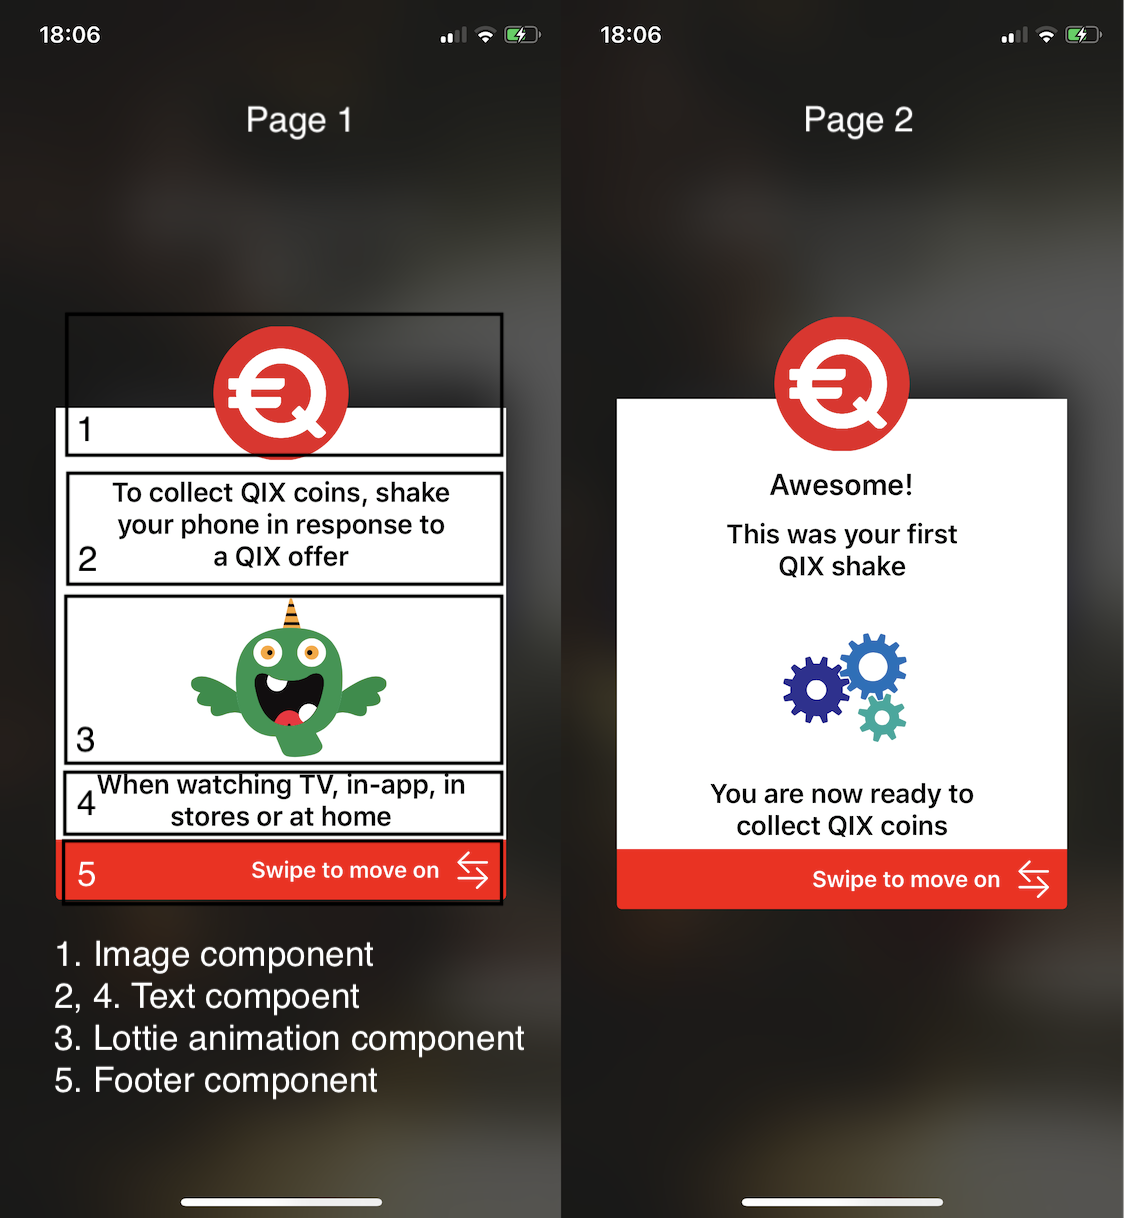
\includegraphics[width=10cm]{an12}
%     \captionof{figure}{
%        CardViews modulari
%     }
%     \label{fig:7}
% \end{minipage}\\


% % % % % % % % % % % % % % % % % % % % % % % % % % % % % % % % % % % % % %
% %                   La paginazione delle animazioni                     %
% % % % % % % % % % % % % % % % % % % % % % % % % % % % % % % % % % % % % %
% \subsection{~\ref{animationenum:5}. Paginazione delle animazioni}

% Avendo definito al punto~\ref{animationenum:1} l'utilizzo di un solo UIViewController per le animazioni da un lato viene semplificata
% la presentazione delle stesse, dato che basterà presentare un solo UIViewController, ma dall'altro verrà delegata
% l'intera paginagione al view controller. \\

% In particolare questo UIViewController accetta come variabile di inizializzazione
% un array di pagine e in base allo stato della UIPanGestureRecognir deciderà se passare alla pagina successiva
% o interrompere l'animazione;

% % % % % % % % % % % % % % % % % % % % % % % % % % % % % % % % % % % % % %
% %                   La paginazione delle animazioni                     %
% % % % % % % % % % % % % % % % % % % % % % % % % % % % % % % % % % % % % %
% \subsection{~\ref{animationenum:5}. Il Collider}

% Come accennato al punto~\ref{animationenum:3} ogni le CardView hanno dei comportamenti fisici definiti
% da UIkit Dynamics, in particolare per conferire un effetto di collisione viene usato un \textbf{UICollisionBehavior} e implementato come segue:

% \begin{minted}{swift}
%     let itemsCollisionBehavior = UICollisionBehavior(items: page.views)
% \end{minted}

% In questo modo ogni ogni oggetto con questo
% comportamento riuscirà a scontrasi con gli altri oggetti simili.

% \section{Tipologie di autenticazione e Firebase}

% Per la progettazionde dell'autenticazione di è voluto ricorrere a qualcosa di 
% già pronto per velocizzare i tempi di sviluppo e quindi evitare di progettare e implementare un sistema 
% complesso come la gestione di utenti non autenticati (Guest).

% Cercando in rete abbiamo optato per l'utilizzo di \textbf{Firebase}\cite{firebase}: ossia una piattaforma
% di sviluppo per applicazione mobili e web acquisita di Google nel 2014. 
% Uno dei motivi fondamentali per cui è stata scelta è la grande quantità di servizi utili come
% analisi dei Crash, tracking della naviazione degli utenti, DynamicLinks (si veda sezione~\ref{section:dynamiclinks})
% e ovviamente l'autenticazione.

% Esistono 3 tipologie di autenticazione come definito nel requisito, ognuna della quali è un'estensione
% di quella precedente: un utente che apre per la prima volta l'applicazione verrà subito registrato 
% come utente anonimo e quindi in \textbf{Trial Mdoe}, se poi decide di effettuare la registrazione può inserire 
% il suo numero di telefono o la sua email e attraverso Firebase l'utente anonimo evolverà in un utente con più
% informazioni, in \textbf{Signed Mode}.

% Successivamente ci sarà nell'applicazione una sezione specifica dove l'utente potrà inserire nuovi dati come nome, cognome e data di nascita
% o semplicemente potrà linkare un social media come Facebook, Google o Instagram. In questo caso l'utente evolverà nuovamente 
% e arriverà nella \textbf{Pro Mode}.

% Il pacchetto Firebase Auth infatti include tutte queste funzionalità e attraverso delle semplici API
% è possibile utilizzarlo come segue:

% Inizializzazione di Firebase nel file di inizializzazione dell'applicazione ossia l'AppDelegate.swift

% \begin{minted}{swift}
%     FirebaseApp.configure()
% \end{minted}

% Creazione di un utente anonimo

% \begin{minted}{swift}
%     Auth.auth().signInAnonymously() { (authResult, error) in
%         // ...
%     }
% \end{minted}

% Collegamento di un account anonimo con numero di telefono o email

% \begin{minted}{swift}
%     // L'oggetto user è sempre disponibile in firebase e
%     // salvato nel keychain di iOS
%     let user = Auth.auth().currentUser

%     // Creazione dell'oggetto credenzial da collegare
%     // all'utente attuale (anonimo o non)
%     let credential = EmailAuthProvider.credential(withEmail: email,
%         password: password)

%     // Linking dei due account
%     user?.link(with: credential) { (authResult, error) in
%         // ...
%     }
% \end{minted}

% Il linking con un qualunque social media è simile all'esempio riportato
% qui sopra, cambiare soltanto il Provider delle credenziali

% \section{I Dynamic Links}\label{section:dynamiclinks}

% Un'altra interessante funzione di Firebase sono i Dynamic Links
% ossia dei semplici URL generati dalla console o generati direttamente dell'applicazione
% che consentono l'iniezione di un altro url a cui l'utente verrà reindirizzato.

% Questo permette agli utenti di aprire direttamente l'applicazione in questione
% attraverso lo smartphone o il Computer attraverso il browser, ma trasportando dei dati utili all'azienda.

% In particolare nel mio caso mi è statp chiesto di implementare un sistema di inviti, per cui 
% un utente può invitarene un altro attraverso questi links.

